\documentclass[conference]{IEEEtran}
\IEEEoverridecommandlockouts

\usepackage[T1]{fontenc}
\usepackage[utf8]{inputenc}
\usepackage[croatian]{babel}
\usepackage{cite}
\usepackage{amsmath,amssymb,amsfonts}
\usepackage{algorithmic}
\usepackage{graphicx}
\usepackage{textcomp}
\usepackage{xcolor}
\def\BibTeX{{\rm B\kern-.05em{\sc i\kern-.025em b}\kern-.08em
    T\kern-.1667em\lower.7ex\hbox{E}\kern-.125emX}}

\begin{document}

\title{Detekcija oštećenja kolnika
}

\author{
\IEEEauthorblockN{1\textsuperscript{st} Josipa Sever}
\IEEEauthorblockA{\textit{Faculty of Electrical Engineering and Computing (FER)} \\
University of Zagreb, Croatia \\
josipa.sever@fer.hr}
\and
\IEEEauthorblockN{2\textsuperscript{nd} Josip Despot}
\IEEEauthorblockA{\textit{Faculty of Electrical Engineering and Computing (FER)} \\
University of Zagreb, Croatia \\
josip.despot@fer.hr}
\and
\IEEEauthorblockN{3\textsuperscript{rd} Nikola Marić}
\IEEEauthorblockA{\textit{Faculty of Electrical Engineering and Computing (FER)} \\
University of Zagreb, Croatia \\
nikola.maric@fer.hr}
\and
\IEEEauthorblockN{4\textsuperscript{th} Franjo Vuković}
\IEEEauthorblockA{\textit{Faculty of Electrical Engineering and Computing (FER)} \\
University of Zagreb, Croatia \\
franjo.vukovic2@fer.hr}
\and
\IEEEauthorblockN{5\textsuperscript{th} Josipa Udovičić}
\IEEEauthorblockA{\textit{Faculty of Electrical Engineering and Computing (FER)} \\
University of Zagreb, Croatia \\
josipa.udovicic@fer.hr}
}


\maketitle



%--- SAŽETAK / ABSTRACT --------------------------------------------------------

% Sažetak na hrvatskom


% Sadržaj se automatski generira / Table of contents is automatically generated

%--- UVOD / INTRODUCTION -------------------------------------------------------
\section{Uvod}
\label{pog:uvod}

Održavanje cestovne infrastrukture jedan je od ključnih čimbenika za sigurnost i učinkovitost cestovnog prometa. Kvaliteta kolnika izravno utječe na sigurnost sudionika u prometu, dugovječnost vozila te ukupne troškove održavanja prometnica. Tradicionalne metode inspekcije kolnika često su vremenski zahtjevne, skupe i podložne subjektivnim procjenama. S obzirom na sve veću dostupnost digitalnih tehnologija i porast količine vizualnih podataka, automatizacija procesa detekcije oštećenja na kolnicima nameće se kao logičan i nužan korak prema modernizaciji cestovnog nadzora.

Tema ovog projekta usmjerena je na razvoj sustava za automatsku detekciju oštećenih dijelova kolnika na temelju analiza digitalnih slika. Detekcija će se ostvariti primjenom metoda digitalne obrade slike u kombinaciji sa strojnim učenjem, pri čemu je naglasak na treniranju modela sposobnog za prepoznavanje oštećenja poput pukotina, rupa i neravnina. Proces uključuje izradu i obradu skupa podataka koji sadrži slike kolnika u različitim stanjima, a za treniranje modela koristit će se konvolucijske neuronske mreže (CNN), koje su se pokazale iznimno učinkovitima u zadacima računalnog vida.

Evaluacija razvijenog modela provodit će se pomoću standardnih metrika kao što su točnost, preciznost i F1-mjera, s ciljem postizanja visoke razine pouzdanosti u stvarnim uvjetima primjene. Na taj način, projekt ne samo da doprinosi razvoju suvremenih tehnoloških rješenja u prometnoj infrastrukturi, već i otvara mogućnosti za njihovu širu implementaciju u sustavima pametnih gradova i automatiziranog upravljanja prometnicama.

%-------------------------------------------------------------------------------
\section{Pregled postojećih pristupa detekciji oštećenja kolnika}
\label{pog:pregled}

Automatska detekcija oštećenja na kolnicima posljednjih je godina postala važno područje istraživanja, potaknuto potrebom za bržim, preciznijim i ekonomičnijim metodama održavanja cestovne infrastrukture. Tradicionalne metode oslanjaju se na vizualne inspekcije koje su često subjektivne, skupe i vremenski zahtjevne, zbog čega se razvijaju računalni sustavi temeljenim na obradi slike i strojnome učenju.

Prvi pristupi ovom problemu koristili su klasične tehnike digitalne obrade slike, uključujući metode binarizacije, morfoloških operacija i detekcije rubova. Iako jednostavne za implementaciju, te metode često podliježu pogreškama u uvjetima lošeg osvjetljenja i šuma u pozadini slike (npr. zbog sjena, ulja ili prljavštine), što ograničava njihovu upotrebljivost u stvarnim uvjetima \cite{lau2020}.

S napretkom dubokog učenja i računalnog vida, značajna pažnja posvećena je primjeni konvolucijskih neuronskih mreža (CNN), koje su se pokazale iznimno učinkovitima u zadacima detekcije i segmentacije oštećenja. Primjerice, U-Net arhitektura korištena je za segmentaciju pukotina na slikama kolnika, pri čemu je postignuta visoka točnost segmentacije i otpornost na šumove \cite{lau2020}.

U daljnjim istraživanjima, autori su primijenili različite CNN arhitekture poput VGG16, ResNet-50 i MobileNet kako bi se usporedila njihova učinkovitost u klasifikaciji oštećenja. Rezultati su pokazali da duboki modeli poput ResNet-a postižu veću preciznost i stabilnost u klasifikaciji pukotina, čak i na različitim skupovima podataka \cite{tapamo2023}.

Za zadatke detekcije u stvarnom vremenu posebno su se pokazali korisnima modeli iz YOLO (You Only Look Once) obitelji, poput YOLOv5 i YOLOv8. Ovi modeli omogućuju brzo i precizno prepoznavanje različitih vrsta oštećenja (npr. pukotine, rupe) uz visoku razinu robusnosti na različitim vrstama podloge i u uvjetima promjenjivog osvjetljenja \cite{nafaa2024}.

Uz obradu RGB slika, sve više istraživanja koristi fuziju podataka iz različitih izvora za poboljšanje detekcije. Primjerice, kombinacijom RGB i termalnih (infracrvenih) slika moguće je bolje razlikovati oštećenja od sjena ili mrlja, čime se smanjuje broj lažno pozitivnih detekcija. U jednom radu postignuta je točnost od 98,34 \% korištenjem EfficientNetB4 modela za analizu kombiniranih slika \cite{mdpi2022}.

Još napredniji sustavi koriste dodatne senzore, poput inercijskih mjernih jedinica (IMU), za prikupljanje podataka o vibracijama vozila. Spajanjem vizualnih podataka s podacima o vibracijama pomoću dubokih modela poput YOLOv7 i Bi-LSTM mreža, moguće je detektirati i dublje oštećenje kolnika koje nije nužno vidljivo na slici \cite{hsieh2024}.

Konačno, pregled literature koji su proveli Guan i suradnici nudi sveobuhvatan prikaz trenutačnih istraživanja na području automatske detekcije cestovnih oštećenja. U radu se detaljno analiziraju pristupi koji koriste podatke iz bespilotnih letjelica, 3D rekonstrukcija terena te izazovi skalabilnosti i generalizacije modela u stvarnim prometnim uvjetima \cite{guan2023}.

% -------------------------------------------------------------------------------

\section{Razvoj i implementacija sustava za detekciju oštećenja na kolnicima}
\label{pog:razvoj}

U nastavku se detaljno opisuje pristup razvijen od strane projektnog tima, uključujući strukturu skupa podataka, arhitekture modela, načine obrade podataka i evaluaciju performansi.

\subsection{Priprema i struktura podataka}
\label{sub:priprema_podataka}

Za potrebe treniranja i evaluacije modela projektni tim koristio je skup podataka \textit{Pothole Detection} dostupan na Roboflow platformi \cite{roboflow_pothole}. Skup se sastoji od kvalitetno anotiranih slika kolnika koje prikazuju različite vrste oštećenja, s jasno označenim bounding boxovima. Ove oznake omogućuju modelima detekcije učenje specifičnih vizualnih karakteristika oštećenja poput pukotina, udubljenja i rupa.

Skup podataka preuzet je i prilagođen za uporabu u YOLO formatu, što podrazumijeva odvojene \texttt{.txt} datoteke za svaku sliku s koordinatama oznaka. Podaci su organizirani u tri glavne skupine:

\begin{itemize}
    \item \textbf{Trening skup (train/)} – služi za učenje modela.
    \item \textbf{Validacijski skup (valid/)} – koristi se za nadzor nad generalizacijskom sposobnošću tijekom treniranja.
    \item \textbf{Testni skup (test/)} – neovisno se koristi za konačnu provjeru učinkovitosti modela.
\end{itemize}

Kako bi se povećala raznolikost i robusnost modela, provedena je i \textbf{augmentacija slika} (rotacija, zrcaljenje, skaliranje, promjene kontrasta i svjetline) uz pomoć Roboflowovih ugrađenih alata. Time se osigurava otpornost modela na promjene u osvjetljenju, perspektivi i teksturi kolnika.

\subsection{Odabrani modeli i pristupi}
\label{sub:odabrani_modeli}

Kako bi se osigurala što viša preciznost u detekciji oštećenja, projektni tim implementirao je više različitih modela, uključujući:

\begin{itemize}
    \item \textbf{Vlastita CNN arhitektura} \\
    Razvijena je prilagođena konvolucijska neuronska mreža (Custom CNN) sa slojevima za ekstrakciju značajki i klasifikaciju, prikladna za rad s manjim skupovima podataka i jednostavnijom strukturom.
    \begin{figure}[htbp]
    \centerline{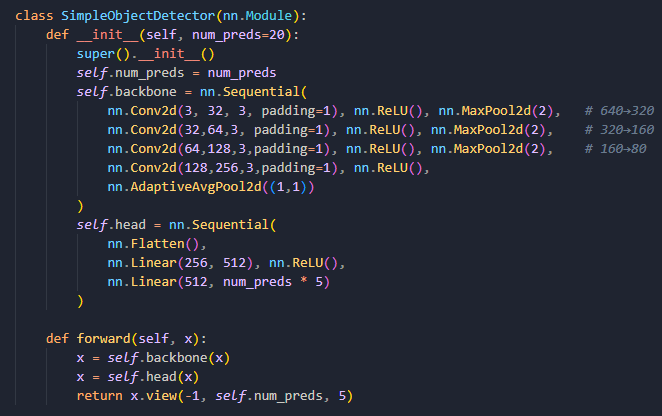
\includegraphics[width=0.45\textwidth]{Images/CustomCNN.png}}
    \caption{Arhitektura vlastite konvolucijske neuronske mreže (Custom CNN), dizajnirana za jednostavnije zadatke detekcije i rad na ograničenim skupovima podataka.}
    \label{fig:customcnn}
    \end{figure}

    \item \textbf{Faster R-CNN} \\
    Primijenjen je napredni model za detekciju objekata koji koristi regijske prijedloge (Region Proposal Network) za identifikaciju potencijalnih područja oštećenja. Ovaj model omogućuje visoku točnost detekcije, ali je računalno zahtjevniji.
    %\begin{figure}[htbp]
    %\centerline{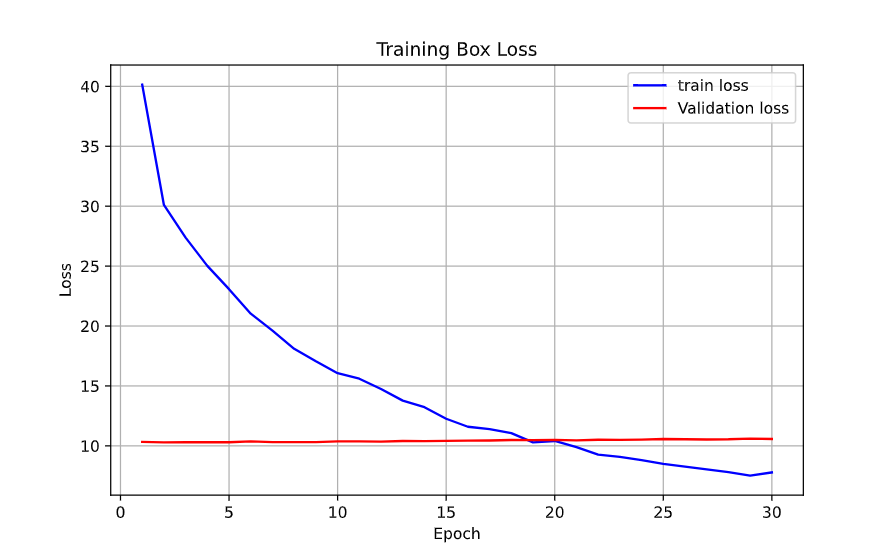
\includegraphics[width=0.45\textwidth]{Images/FasterCNN.jpg}}
    %\caption{Vizualni prikaz Faster R-CNN modela, koji koristi regijske prijedloge za identifikaciju potencijalnih područja oštećenja.}
    %\label{fig:fasterrcnn}
    %\end{figure}

    \item \textbf{YOLOv8} \\
    Model YOLOv8 implementiran je kao najučinkovitije rješenje za detekciju u stvarnom vremenu. Njegova brzina izvođenja i visoka preciznost čine ga izuzetno pogodnim za primjene u stvarnom okruženju, kao što su mobilne aplikacije za pregled cesta.
    \begin{figure}[htbp]
    \centerline{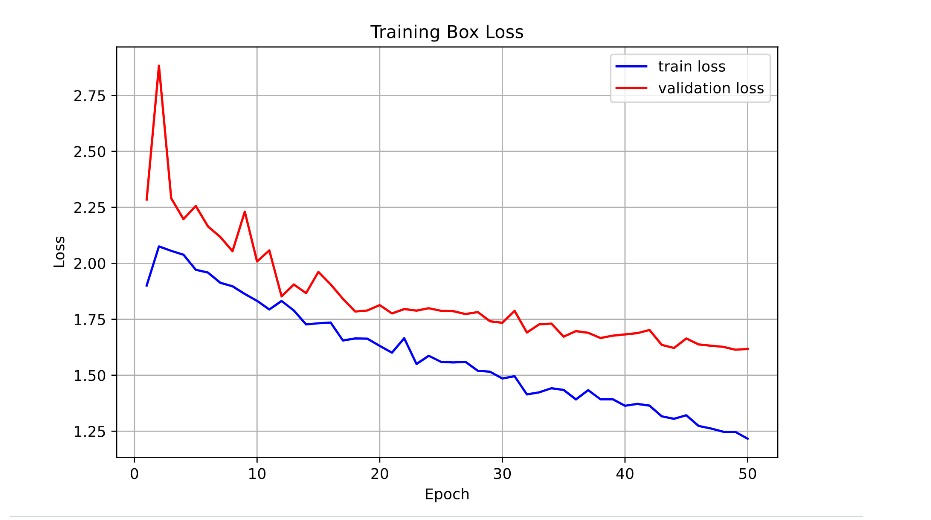
\includegraphics[width=0.45\textwidth]{Images/YOLO.jpg}}
    \caption{YOLOv8 model za detekciju u stvarnom vremenu, s fokusom na efikasnost i brzinu izvođenja.}
    \label{fig:yolo}
    \end{figure}
\end{itemize}

\subsection{Treniranje i evaluacija modela}
\label{sub:treniranje_evaluacija}

Svi modeli trenirani su koristeći unaprijed pripremljeni skup podataka, pri čemu su korištene različite strategije augmentacije slika (npr. rotacija, zrcaljenje, promjene kontrasta) radi povećanja raznolikosti ulaznih podataka. Parametri treniranja (broj epoha, veličina batcha, stopa učenja) prilagođeni su svakom modelu kako bi se postigli optimalni rezultati.

Evaluacija performansi provedena je korištenjem standardnih metrika:

\begin{itemize}
    \item \textbf{Preciznost (precision)} – omjer ispravno detektiranih oštećenja i svih detekcija.
    \item \textbf{Odziv (recall)} – omjer ispravno detektiranih oštećenja i ukupnog broja stvarnih oštećenja.
    \item \textbf{F1-mjera} – harmonijska sredina preciznosti i odziva.
    \item \textbf{mAP (mean Average Precision)} – mjerilo koje kombinira preciznost i lokalizaciju objekata kroz različite pragove.
\end{itemize}

Rezultati evaluacije prikazani su grafički i tablično te su korišteni za usporedbu performansi između modela.

%-------------------------------------------------------------------------------

\section{Opis eksperimentalnih rezultata}

U ovom poglavlju prikazani su i analizirani rezultati eksperimenta provedenog u svrhu detekcije oštećenja na kolniku pomoću različitih modela dubokog učenja. Evaluacija se temeljila na usporedbi predikcija s referentnim (engl. \textit{ground truth}) oznakama, pri čemu su korištene standardne metrike poput točnosti (\textit{accuracy}), preciznosti (\textit{precision}), odziva (\textit{recall}) i F1-mjere. Testirani su sljedeći modeli: YOLO, Faster R-CNN i vlastiti (custom) konvolucijski neuronski model.

\subsection{Rezultati modela YOLO}

Model YOLO (\textit{You Only Look Once}), poznat po svojoj brzini i efikasnosti u detekciji objekata, pokazao je ograničene rezultate u ovom eksperimentu. Tijekom treniranja zabilježen je pad vrijednosti funkcije gubitka (\textit{loss}), što ukazuje na učenje modela.

\textbf{Evaluacijski rezultati za YOLO model:}
\begin{itemize}
  \item \textbf{Preciznost:} 0{,}5757
  \item \textbf{Odziv:} 0{,}4376
  \item \textbf{F1 mjera:} 0{,}4972
  \item \textbf{Točnost:} 0{,}4637
\end{itemize}

Iako je YOLO postigao relativno solidnu preciznost, nizak odziv sugerira da model često propušta detektirati stvarna oštećenja. Time se smanjuje njegova pouzdanost u kontekstu prometne sigurnosti.

\begin{figure}[htbp]
\centerline{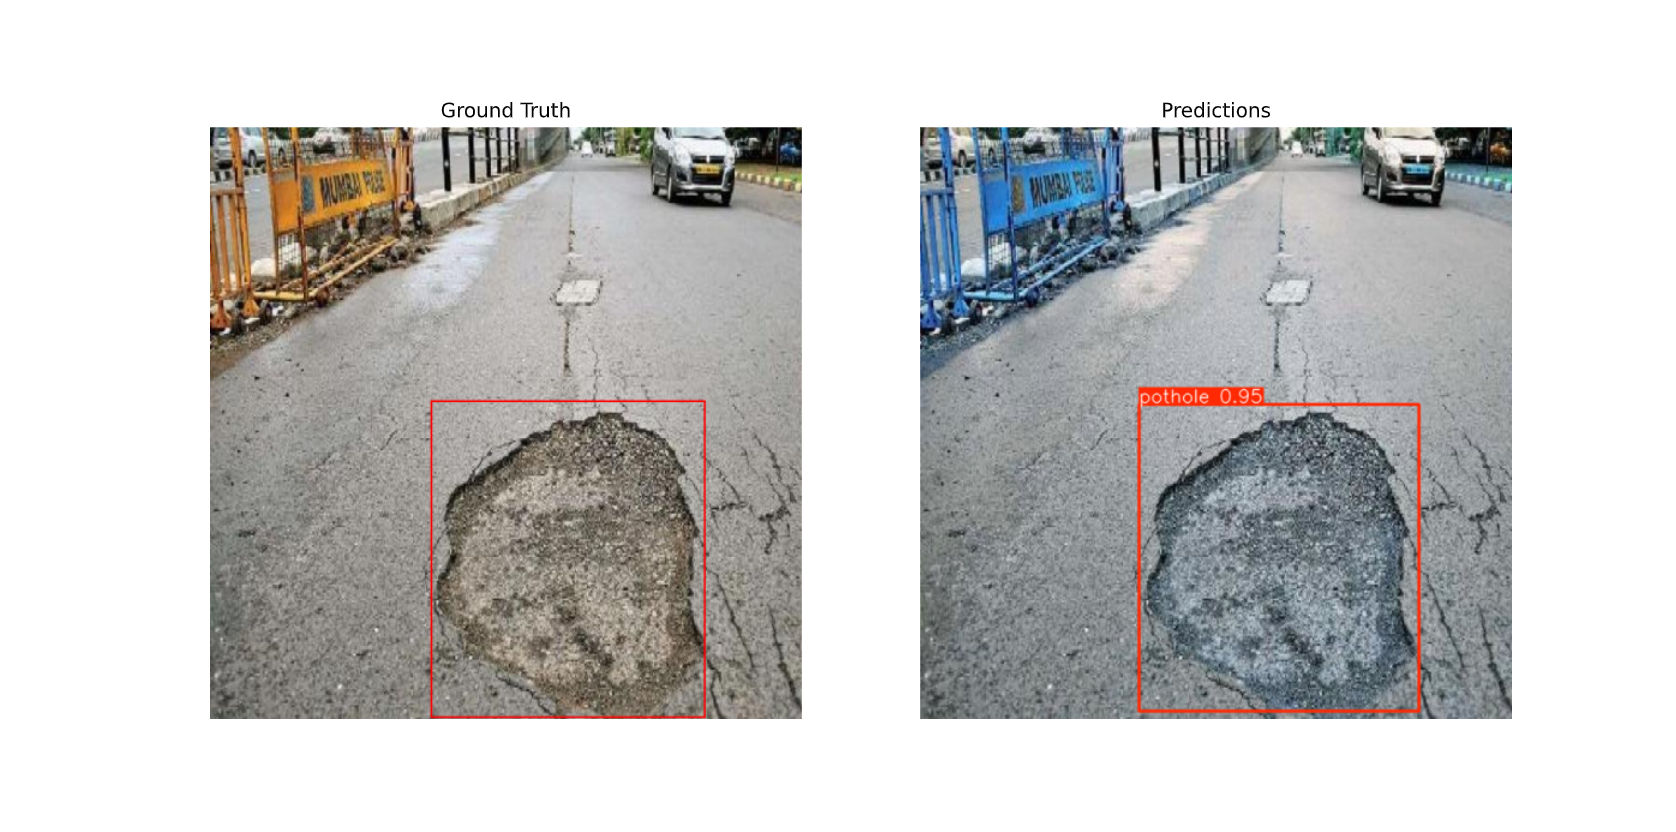
\includegraphics[width=0.48\textwidth]{Images/YOLOPic.png}}
\caption{Točna i pouzdana detekcija oštećenja na cesti korištenjem YOLO modela. Model precizno lokalizira pothole s confidence score 0.95.}
\label{fig:yolo_eval}
\end{figure}

\subsection{Rezultati modela Faster R-CNN}

Faster R-CNN je kompleksniji model poznat po visokoj preciznosti. U eksperimentima je pokazao značajno bolje rezultate u odnosu na YOLO.

\textbf{Evaluacijski rezultati za Faster R-CNN model:}
\begin{itemize}
  \item \textbf{Prosječan odziv:} 0{,}7425
  \item \textbf{Prosječna preciznost:} 0{,}5733
\end{itemize}

Vrijednosti funkcije gubitka su se stabilno smanjivale tijekom epoha, a model je uspješno detektirao različite vrste oštećenja, uključujući i manja i slabije vidljiva oštećenja na površini kolnika.

\begin{figure}[htbp]
\centerline{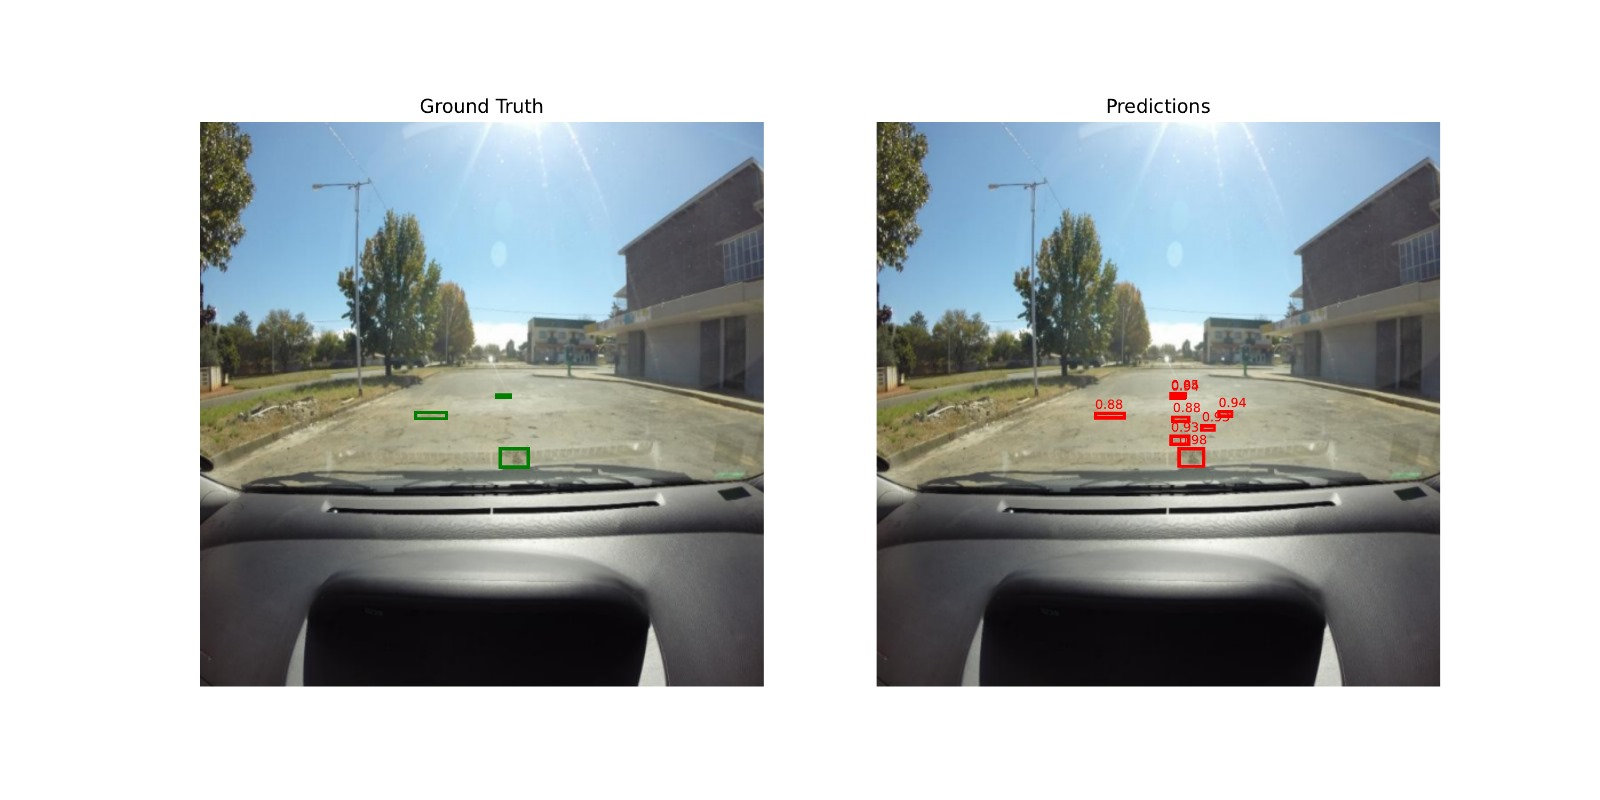
\includegraphics[width=0.48\textwidth]{Images/FasterCNNPic.jpg}}
\caption{Primjer gdje Faster R-CNN model generira više predikcija, od kojih su mnoge točne (visoka preciznost, ali uz pojavu lažno pozitivnih).}
\label{fig:fasterrcnn_eval}
\end{figure}


\subsection{Rezultati vlastitog konvolucijskog modela}

Vlastiti konvolucijski neuronski model razvio se u okviru rada s ciljem testiranja prilagođene arhitekture. Iako su u nekim slučajevima predikcije bile usporedive s referentnim oznakama, ukupna učinkovitost bila je znatno manja u odnosu na prethodna dva modela.
Zbog nedostatka formalnih evaluacijskih metrika, analiza se oslanjala na vizualnu procjenu točnosti, koja je pokazala značajnu osjetljivost modela na šum i promjene u uvjetima osvjetljenja.

\begin{figure}[htbp]
\centerline{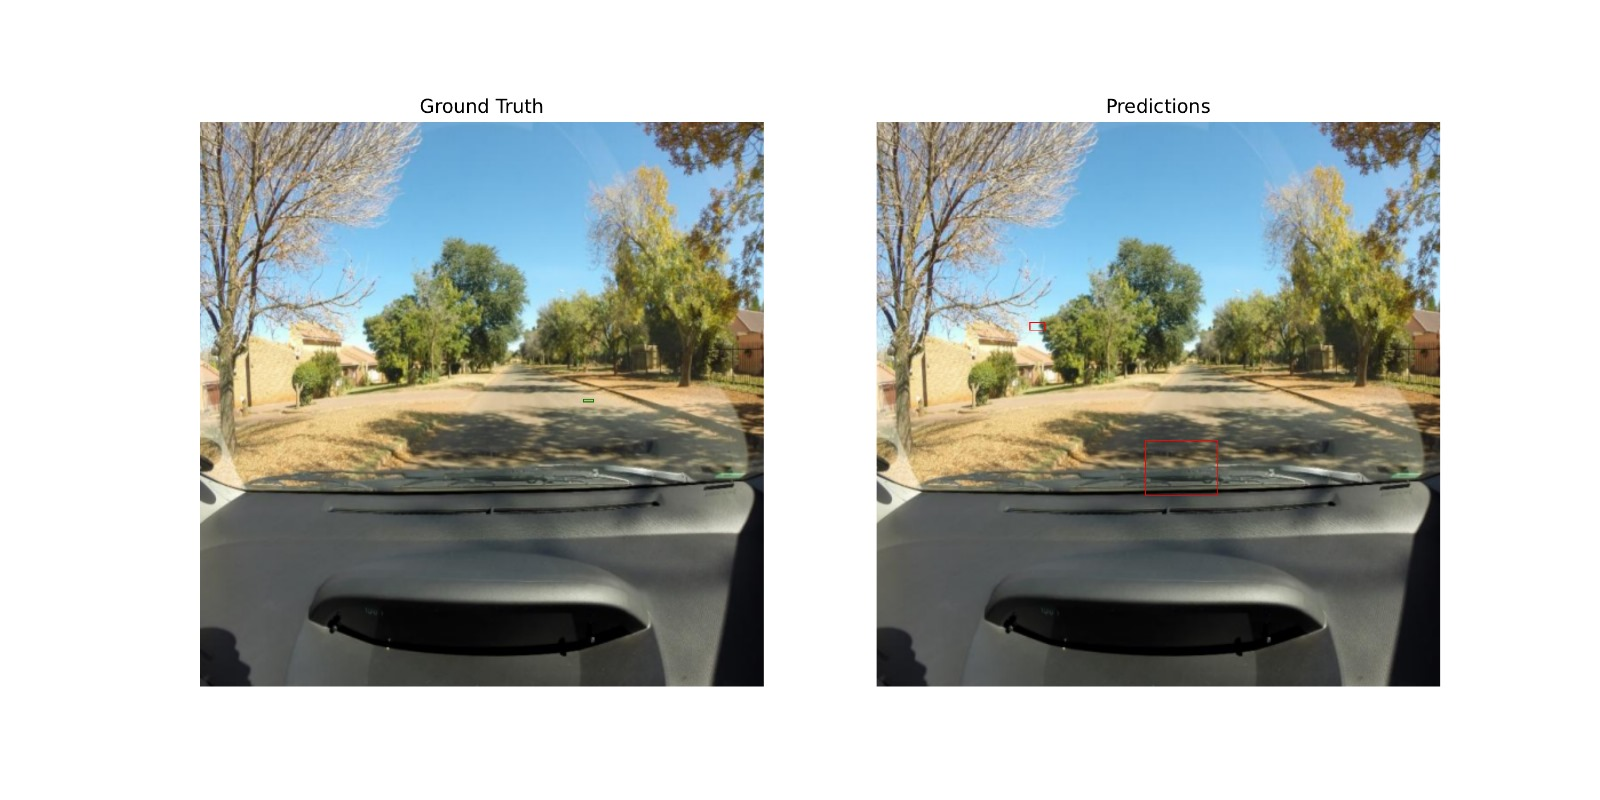
\includegraphics[width=0.48\textwidth]{Images/CustomCNNPic.jpg}}
\caption{Usporedba između stvarnih oznaka (Ground Truth) i predikcija vlastitog CNN modela. Primjećuje se netočna lokalizacija oštećenja.}
\label{fig:customcnn_eval}
\end{figure}

\subsection{Vizualizacija predikcija}

Vizualna usporedba predikcija i referentnih oznaka dodatno ilustrira razlike među modelima. Faster R-CNN se pokazao najkonzistentnijim u prostornom poklapanju s oznakama. Kod YOLO-a su uočene pogreške u obliku lažno pozitivnih i negativnih detekcija, dok je vlastiti model nerijetko davao nepotpune ili netočne rezultate.

%---------------------------------------------------------------------------------

\section{Diskusija i Usporedba s Postojećim Radovima}
U ovom poglavlju analiziramo rezultate našeg modela za detekciju oštećenja na kolnicima te ih uspoređujemo s prethodnim istraživanjima navedenima u literaturi. Poseban fokus je stavljen na metrike točnosti (precision), odziva (recall), F1 rezultata i ukupne točnosti modela, kao i na korištene arhitekture i podatkovne skupove.

\subsection{Usporedba s Modelima iz Literature}

\subsubsection*{YOLO model}

U našem eksperimentu, YOLO model je postigao sljedeće metrike:
\begin{itemize}
    \item \textbf{Preciznost}: 0.5757
    \item \textbf{Odziv}: 0.4376
    \item \textbf{F1 rezultat}: 0.4972
    \item \textbf{Točnost}: 0.4637
\end{itemize}

U radu Nafaa et al. (2024) \cite{nafaa2024}, koji također koristi YOLO pristup, autori ne navode identične metrike, ali prijavljuju visoku učinkovitost klasifikacije pukotina s naglaskom na detekciju u stvarnom vremenu. Usporedno, naši rezultati su nešto niži, što se može pripisati različitostima u veličini i kvaliteti skupa podataka, verziji YOLO modela te eventualnom nedostatku dodatnih augmentacijskih tehnika.

\subsubsection*{Faster R-CNN model}

Faster R-CNN u našim testovima pokazao se kao model s:
\begin{itemize}
    \item \textbf{Prosječnim odzivom (recall)}: 0.7425
    \item \textbf{Prosječnom preciznošću}: 0.5733
\end{itemize}

U usporedbi s radom Hsieh et al. (2024) \cite{hsieh2024}, gdje se koristi kombinacija YOLOv7 i BiLSTM modela u višemodalnom okruženju (RGB + Lidar), njihova arhitektura rezultira višom točnošću. Naš model se približava njihovim rezultatima u pogledu preciznosti, iako ne koristi dodatne senzorske informacije, što ukazuje na snažnu generalizacijsku sposobnost.

\subsubsection*{Custom CNN model}

Custom CNN arhitektura u našem radu nije dala dovoljno kvantitativnih metrika za izravnu usporedbu. Ipak, vizualna evaluacija predikcija pokazuje više pogrešaka u odnosu na YOLO i Faster R-CNN modele, što je očekivano s obzirom da jednostavni CNN modeli često nemaju dovoljan kapacitet za zahtjevne zadatke poput detekcije pukotina.

\subsection{Usporedba sa Širim Radovima}

U preglednom radu Guan et al. (2023) \cite{guan2023}, istaknuto je da detekcija oštećenja na cesti uz pomoć dubokog učenja daje najbolje rezultate kada se koriste složene arhitekture i optimizacija hiperparametara. Naša implementacija Faster R-CNN modela potvrđuje ovu tvrdnju.

Rad Bui et al. (2022) \cite{mdpi2022} koristi fuziju RGB i termalnih slika za poboljšanje detekcije. Budući da u našem radu nije korištena višemodalna obrada, sugerira se mogućnost daljnjeg povećanja preciznosti uvođenjem dodatnih senzorskihpodataka.


%--- ZAKLJUČAK / CONCLUSION ----------------------------------------------------
\section{Zaključak}
\label{pog:zakljucak}

U ovom radu predstavljen je razvoj i evaluacija sustava za automatsku detekciju oštećenja na kolnicima korištenjem dubokih konvolucijskih neuronskih mreža. Korišten je kvalitetno anotirani skup podataka, a razvijeni modeli uspoređeni su s obzirom na točnost, preciznost, odziv i F1-mjeru.

Odabrana su tri različita pristupa: vlastita CNN arhitektura, Faster R-CNN te YOLOv8. Analiza je pokazala da, iako vlastiti model može pružiti osnovne rezultate u ograničenim uvjetima, pokazuje značajna ograničenja u pogledu generalizacije i osjetljiv je na varijacije u ulaznim podacima. YOLOv8 model pokazao je bolju preciznost, ali i ograničen odziv, što znači da često propušta detektirati neka stvarna oštećenja. S druge strane, Faster R-CNN model postigao je najstabilnije i najuravnoteženije rezultate među testiranim arhitekturama, s visokim odzivom i preciznom lokalizacijom oštećenja.

Vizualna analiza dodatno je potvrdila kvantitativne rezultate te ukazala na prednosti i slabosti svakog pristupa u stvarnim uvjetima. Faster R-CNN se pokazao najpouzdanijim za dublju analizu, dok YOLO ostaje vrlo koristan u aplikacijama gdje je vrijeme izvođenja ključno.

Zaključno, rad potvrđuje učinkovitost primjene metoda dubokog učenja u području detekcije cestovnih oštećenja te postavlja temelje za buduće proširenje sustava korištenjem dodatnih izvora podataka (npr. termalne slike, IMU senzori) i optimizaciju modela za rad u stvarnom vremenu. Predložena rješenja mogu imati značajan doprinos u kontekstu pametnih gradova, digitalnog održavanja infrastrukture i poboljšanja prometne sigurnosti.

%--- LITERATURA / REFERENCES ---------------------------------------------------

% Literatura se automatski generira / References are automatically generated
% Upiši ime BibTeX datoteke bez .bib nastavka / Enter the name of the BibTeX file without .bib extension

\begin{thebibliography}{99}
\bibitem{lau2020} Lau, S. and Nguyen, T. and Kim, J., \textit{Automatic Pavement Crack Detection Using U-Net Based Deep Convolutional Neural Network}, 2020. [Online]. Available: https://arxiv.org/abs/2001.01912
\bibitem{tapamo2023} Tapamo, J. R. and Mushonga, M. and Asabere, N. Y., \textit{Performance Comparison of Deep Learning Models for Pavement Crack Detection}, 2023. [Online]. Available: https://arxiv.org/abs/2304.02933
\bibitem{nafaa2024} Nafaa, M. and Wahbi, M. and Zenkouar, K., \textit{YOLO-based Pavement Crack Detection and Classification}, 2024. [Online]. Available: https://arxiv.org/abs/2406.07674
\bibitem{mdpi2022} Bui, D. T. and Le, T. T. H. and Nguyen, Q. T., \textit{Pavement Defect Detection Using RGB-Thermal Image Fusion and EfficientNet}, 2022. [Online]. Available: https://doi.org/10.3390/rs14010106
\bibitem{hsieh2024} Hsieh, C. Y. and Liu, C. Y. and Chen, C. L., \textit{A YOLOv7-BiLSTM Based Multimodal Deep Learning Model for Pothole Detection}, 2024. [Online]. Available: https://doi.org/10.3390/info15040239
\bibitem{guan2023} Guan, W. and Xu, X. and Zhao, J., \textit{A Comprehensive Review of Deep Learning Approaches for Road Surface Damage Detection}, 2023. [Online]. Available: https://arxiv.org/abs/2308.00828
\bibitem{roboflow_pothole} Roboflow, \textit{Pothole Detection Dataset}, 
\end{thebibliography}

%--- PRIVITCI / APPENDIX -------------------------------------------------------


\end{document}